\section{Geometrically Attracting or Repelling Fixed Points}
\sectiontitleframe

\begin{frame}{Topologically attracting}
    \begin{definition}The fixed point $\fix$ of $f$ is    called \emph{topologically attracting} if\,   $\exists$\, a neighbourhood $U$ on which the iterates ${f}^{\circ n}$ are defined and converge uniformly to the constant map $z \longmapsto z^*$.
    \end {definition}
\end{frame}    
    
\begin{frame}{Topologically attracting and multiplier }
  
        \begin{theorem}
          Consider the function $f(z)=\lambda z+a_{2} z^{2}+a_{3} z^{3}+\dots$ with fixed point $z^*=0$. Then the origin is topologically attracting iff $\abs{\lambda}<1$.
        \end{theorem}
 
       

\end{frame}
\begin{frame}{Koenigs linerisation}
    \begin{theorem}
    For $ f(z)=\lambda z+a_{2} z^{2}+a_{3} z^{3}+\dots$ such that $\abs{\lambda} \notin \{0,1\}$, there exists a local biholomorphic function $\lin{z}=\linT(z)$ in some neighbourhood $\nhd$ of 0 such that the following diagram commute and $\linT (0)=0$ 
    \begin{figure}
    \centering
    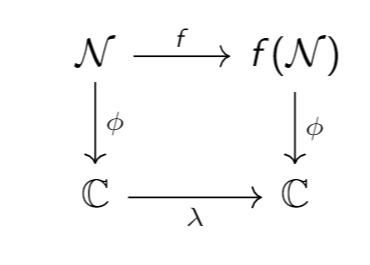
\includegraphics[width=3cm]{resources/ch-08/graph1.png}
   
    \end{figure}

    \end{theorem} 
    Here $ \linT(z)=\lim _{n \tendsto \infty} \iter{f}{n}(z) / \lambda^{n}$
\end{frame}


                    
          

\begin{frame}{Basin of attraction}
    \begin{definition}
        \label{intro:dfn:basin}
        The \emph{attraction basin} $\basin$ of a fixed point $z^*$ is the set of all points that converge to $z^*$ under iterations of $f$
        \begin{equation*}
            \basin(z^*) = \{z_0\mid \lim_{n \rightarrow \infty} \iter{f}{n}(z_0) = z^*\}
        \end{equation*}
        The \emph{immediate basin} $\basin_0$ is the connected component of $\basin$ that contains $z^*$.
    \end{definition}
\end{frame}
\begin{frame}{Global linearisation for a geometrically attracting fixed point}
    \begin{theorem}[Global linearisation] 
        \label{8:thm:attlinglob}
        Up to multiplication by a non-zero constant, there exists a unique local biholomorphic map $\linT:\basin\to\C$ such that the following diagram commute and $\linT(0)=0$.
    \end{theorem}
 
     \begin{figure}
    \centering
    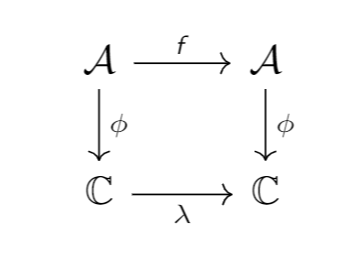
\includegraphics[width=3cm]{resources/ch-08/graph2.png}
    \end{figure} 
    
    We can prove this by defining $\linT(z)=\lambda^{-n}\linT_r(\iter{f}{n}(z))$ where $n$ is the smallest integer for which $\abs{\iter{f}{n}(z)}<r$.
\end{frame}

\begin{frame}{Inverse of linearization and critical point}
    In this lemma consider $f$ is a rational function with degree $\geq 2$ over $\widehat{\C}$ and the fixed point $\fix \in \mathbb{C}$ so that the local behaviour is exactly the same as before.
    \begin{lemma}
    The local inverse in the last theorem $\linV_\eps: \D_{\eps} \to \basin_{0}$ can be uniquely analytically extended to some maximal open disc $\D_{r}$ as $\linV_r: \D_{r} \to \basin_{0}$ with $\linV_r(0)=0$ and $\linT\circ \linV_r(\lin{z}) = \lin{z}$. 
    
    Furthermore, $\linV_r$  can be continuously extended to the boundary $\partial \D_{r}$ and there exists at least one critical point of $f$ in the $\linV_r(\partial \D_{r})$.
    \end{lemma}
\end{frame}

\begin{frame}{Attracting periodic orbit}
    \begin{definition}

        A \emph{periodic orbit} is an orbit $z_0 \rightarrow z_1 \rightarrow z_2 \rightarrow \cdots $ such that $z_m =\iter{f}{m}(z_0)=z_0$ for some integer $m$. A periodic orbit is called \emph{attracting} if the derivative $\abs{\left(\iter{f}{m}\right)'\left(z_{k}\right)}<1$. 
    \end{definition}
    
    Note:  $\abs{\left(\iter{f}{m}\right)'\left(z_{k}\right)}$ is the same for all $z_{k}$.
    
    \begin{definition}
    Since each $z_k$ is a fixed point of $\iter{f}{m}$, they have corresponding immediate basins. The immediate basin $\basin_0(\mathcal{O}, f)$ of a periodic orbit $\mathcal{O}$ is the union of the immediate basins of each point in the orbit under $\iter{f}{m}$.
    \end{definition}
    
\end{frame}

\begin{frame}{Attracting periodic orbit and critical point}
    \begin{theorem}
        For $f$ a nonlinear rational map, the immediate basin of every attracting periodic orbit contains at least one critical point.
    \end{theorem}
    
    Idea of proof: 
    
    \begin{itemize}
        \item $f^{\circ m}$ maps $\basin^{0}\left(z_{j}\right)$ into itself. 
        \item $f$ has no critical point $\implies f^{\circ m}$ no critical point.
        \item Basin of attraction of a attracting fixed point must contain a critical point.
    \end{itemize}
\end{frame}
\begin{frame}{Approximating attracting periodic orbit}
    \begin{cor}
    \label{8:cor:orbfin}
    Such a rational map $f$ has only finitely many attracting periodic orbits.
    \end{cor}   
    
    \textbf{A logarithm for approximating periodic orbit:} 
    
    \begin{itemize}
        \item Locate all critical points of the function
        \item Iteratively apply the function from the critical point.
        \item Observe if it converges to a periodic orbit.
    \end{itemize}
    
    \textbf{Note}: May fail for large period. e.g.$f(z)=z^2-1.5$.
\end{frame}

\begin{frame}{Topologically Repelling}
    \begin{definition}
   
    The fixed point $\fix$ of $f$ is called \emph{topologically repelling} if for some neighbourhood $\nhd$ of $\fix$, $\forall z \in \nhd $ and $z \neq \fix,\; \exists\, n \in \N$ s.t. $\iter{f}{n}\left(z\right)$ leaves $\nhd$.  Here we call $\nhd$ a \emph{forward isolating neighbourhood} of $\fix$.
    \end{definition}
    
    \textbf{Note}: The only orbit that stays in $\nhd$ is the orbit of the fixed point $\fix$.
\end{frame}

\begin{frame}{Topologically repelling and multiplier}
    \begin{theorem}
          Consider the function $f(z)=\lambda z+a_{2} z^{2}+a_{3} z^{3}+\dots$ with fixed point $z^*=0$. Then the origin is topologically repelling iff $\abs{\lambda}>1$.
        \end{theorem}
\end{frame}

\begin{frame}{generlization of $\linV_{\epsilon}$ in repelling case}
    \begin{thm}
    For a repelling fixed point of $f$, there exists an entire bijective function $\linV$ such that $\linV (0)=0$ and $\linV$ conjugates $f$ to the linear map $\lin{z} \mapsto \lambda\lin{z}$. Moreover, $\linV$ is unique (up to multiplication by a non-zero constant).
     \begin{figure}
    \centering
    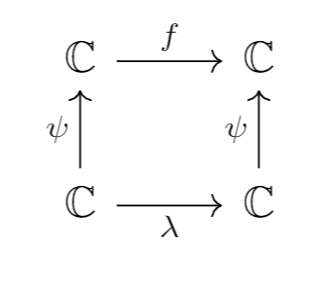
\includegraphics[width=3cm]{resources/ch-08/graph3.png}
   
    \end{figure}
    \end{thm} 
   
   \textbf{Idea of proof}: 
   
   Choose the smallest $n$  such that $z/{\lambda ^{n}}\in\D_{\eps}(0)$, then define $\linV(z)=\iter{f}{n}(\linV_{\eps} (z/{\lambda ^{n}}))$.
\end{frame}
